\documentclass[a4paper,11pt, uplatex, dvipdfmx]{jsarticle}
\usepackage{amsmath,amsthm,amssymb,amsfonts,fancyhdr, enumerate, setspace, braket, emathEy, graphicx}

\newcommand{\ds}{\displaystyle}




\chead{9.2  練習問題解答 }
\lhead{}
\rhead{}
\cfoot{}

\pagestyle{fancy}

\begin{document}



\begin{enumerate}[(1)]

  \setlength{\itemsep}{2zh}

\item $\ds \iint_{D} \left( x^2-y^2 \right) \ dx dy, \quad D=\Set{(x,y) \ \mid \ 1 \leqq x +y \leqq 2, \; 0 \leqq x-y \leqq 1}$

  \vspace{1zh}
  
  $u=x+y, \; v= x-y$ とおく.つまり,以下の変数変換を考える.
  \[ 
    \begin{cases}
      x = \frac{1}{2}u + \frac{1}{2}v\\[1ex]
      y = \frac{1}{2}u - \frac{1}{2}v
    \end{cases}
  \]
  これは $uv$ 平面の閉領域
  \[
    E = \Set{(u,v) \ \mid \ 1 \leqq u \leqq 2, \; 0 \leqq v \leqq 1}
  \]
  を $xy$ 平面の閉領域 $D$ に変換する.変換の Jacobian は
  \[
    J(u,v) = \left|
      \begin{array}{cc}
        \frac{\partial x}{\partial u} & \frac{\partial x}{\partial v}\\[1ex]
        \frac{\partial y}{\partial u} & \frac{\partial y}{\partial v}
      \end{array}
    \right| = \left|
      \begin{array}{rr}
        \frac{1}{2} & \frac{1}{2}\\
        \frac{1}{2} & -\frac{1}{2}
      \end{array}
      \right| = -\frac{1}{2}
  \]
  だから,2重積分は次のように計算できる.
  \[
    \iint_{D} \left( x^2-y^2\right) \ dx dy = \iint_{E} uv |J(u,v)| \
    du dv = \frac{1}{2}\left(\int_{1}^{2}u \ du \right) \left(
      \int_{0}^{1} v \ dv \right) =\frac{3}{8}
  \]

    
  \begin{table}[h]
    \centering
    \begin{tabular}[h]{cc}
      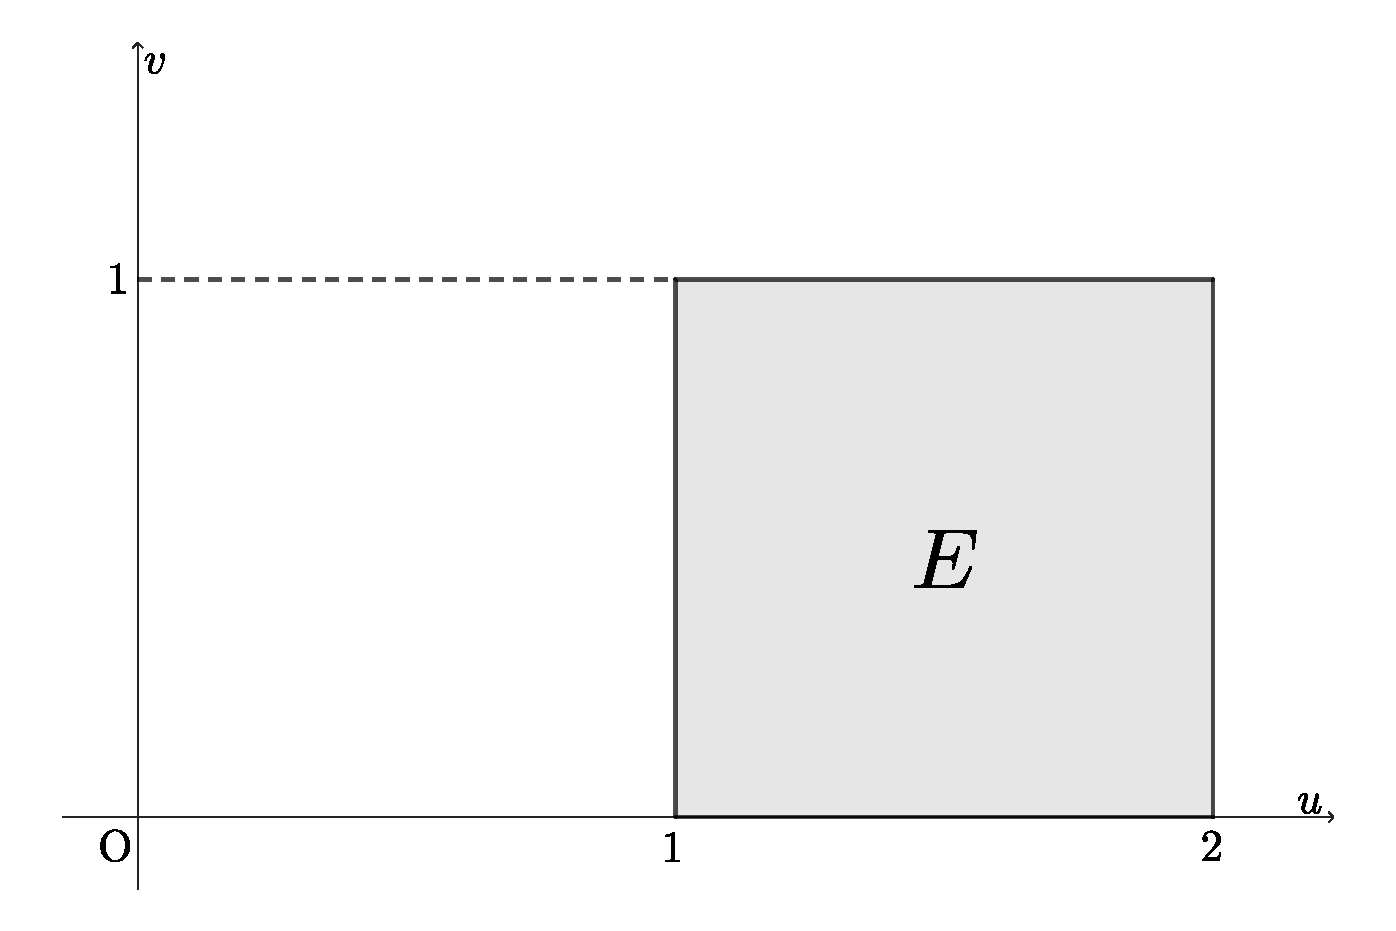
\includegraphics[height=5cm]{./pictures/fig1_uv.pdf} 
      &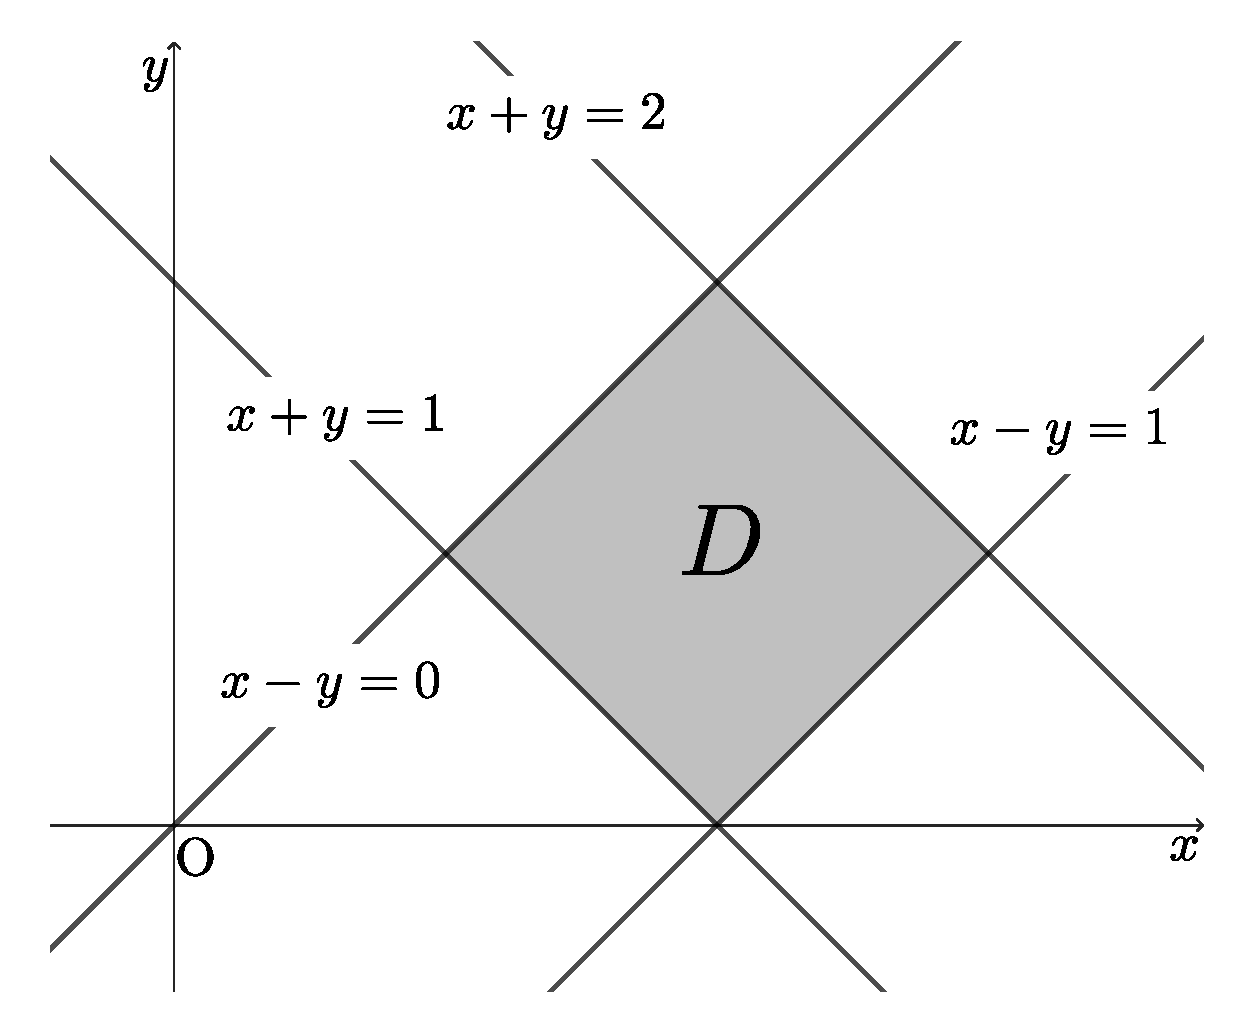
\includegraphics[height=5cm]{./pictures/fig1_xy.pdf}
    \end{tabular}
  \end{table}

  \newpage
  
\item $\ds \iint_{D} e^{-x^2-y^2} \ dx dy, \quad D=\Set{(x,y) \ \mid \ 1 \leqq x^2+y^2 \leqq 9}$

  \vspace{1zh}

  極座標変換 $
  \begin{cases}
    x=r\cos \theta\\
    y=r\sin \theta
  \end{cases}
  $ によって,$r\theta$ 平面の閉領域
  \[
    E = \Set{(r, \theta) \ \mid \ 1 \leqq r \leqq 3, \; 0 \leqq \theta \leqq 2\pi}
  \]
  が $xy$ 平面の閉領域 $D$ に変換される.極座標変換の Jacobian は
  \[
    J(r, \theta) = \left|
      \begin{array}{rr}
        \cos \theta & -r \sin \theta\\
        \sin \theta & r \cos \theta
      \end{array}
    \right| = r \left( \cos^2 \theta + \sin^2 \theta\right) = r
  \]
  なので,2重積分は次のように計算できる.
  \[
    \iint_{D} e^{-x^2 -y^2} \ dx dy = \iint_{E} e^{-r^2} \left|
      J(r,\theta)\right| = \left(\int_{0}^{2\pi} \ d\theta\right)
    \left( \int_{1}^{3} re^{-r^2} \ dr\right) = \pi \left(
      e^{-1}-e^{-9}\right) 
  \]
  
  \begin{table}[h]
    \centering
    \begin{tabular}[h]{cc}
      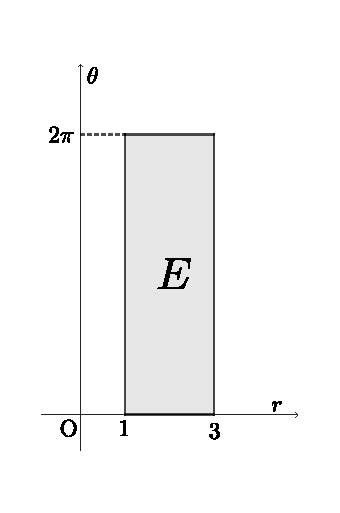
\includegraphics[height=8cm]{./pictures/fig2_rt.pdf} 
      &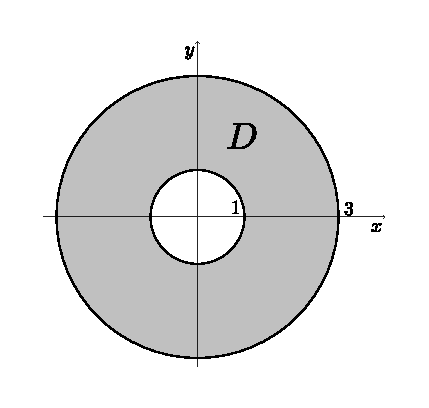
\includegraphics[height=8cm]{./pictures/fig2_xy.pdf}
    \end{tabular}
  \end{table}

  \newpage
  
\item
  $\ds \iint_{D} \sqrt{x^2+y^2} \ dx dy, \quad D=\Set{(x,y) \ \mid \ 0
    \leqq y \leqq x^2+y^2 \leqq 1, \; 0 \leqq x}$

  \vspace{1zh}

  極座標変換 $
  \begin{cases}
    x=r\cos \theta\\
    y=r\sin \theta
  \end{cases}
  $ によって,$r\theta$ 平面の閉領域
  \[
    E = \Set{(r, \theta) \ \mid \ 0 \leqq \theta \leqq \frac{\pi}{2}, \; \sin \theta \leqq r \leqq 1}
  \]
  が $xy$ 平面の閉領域 $D$ に変換される.極座標変換
  の Jacobian は前問と同じく
  \[
    J(r,\theta)=r
  \]
  なので,2重積分は次のように計算できる.
  \[
    \begin{aligned}
      \iint_{D}\sqrt{x^2+y^2} \ dx dy
      &= \iint_{E} \sqrt{r^2} \left| J(r, \theta) \right| \ dr d\theta
        =  \int_{0}^{\pi/2} \left( \int_{\sin \theta}^{1} r^2 \ dr \right) d\theta\\[1ex]
      &= \int_{0}^{\pi/2} \left[ \frac{r^3}{3}\right]_{r=\sin\theta}^{r=1} \ d\theta
        = \frac{1}{3} \int_{0}^{\pi/2} \left( 1 - \sin^3 \theta\right) \ d\theta
        = \frac{\pi}{6} - \frac{2}{9}
    \end{aligned}
  \]

  \begin{table}[h]
    \centering
    \begin{tabular}[h]{cc}
      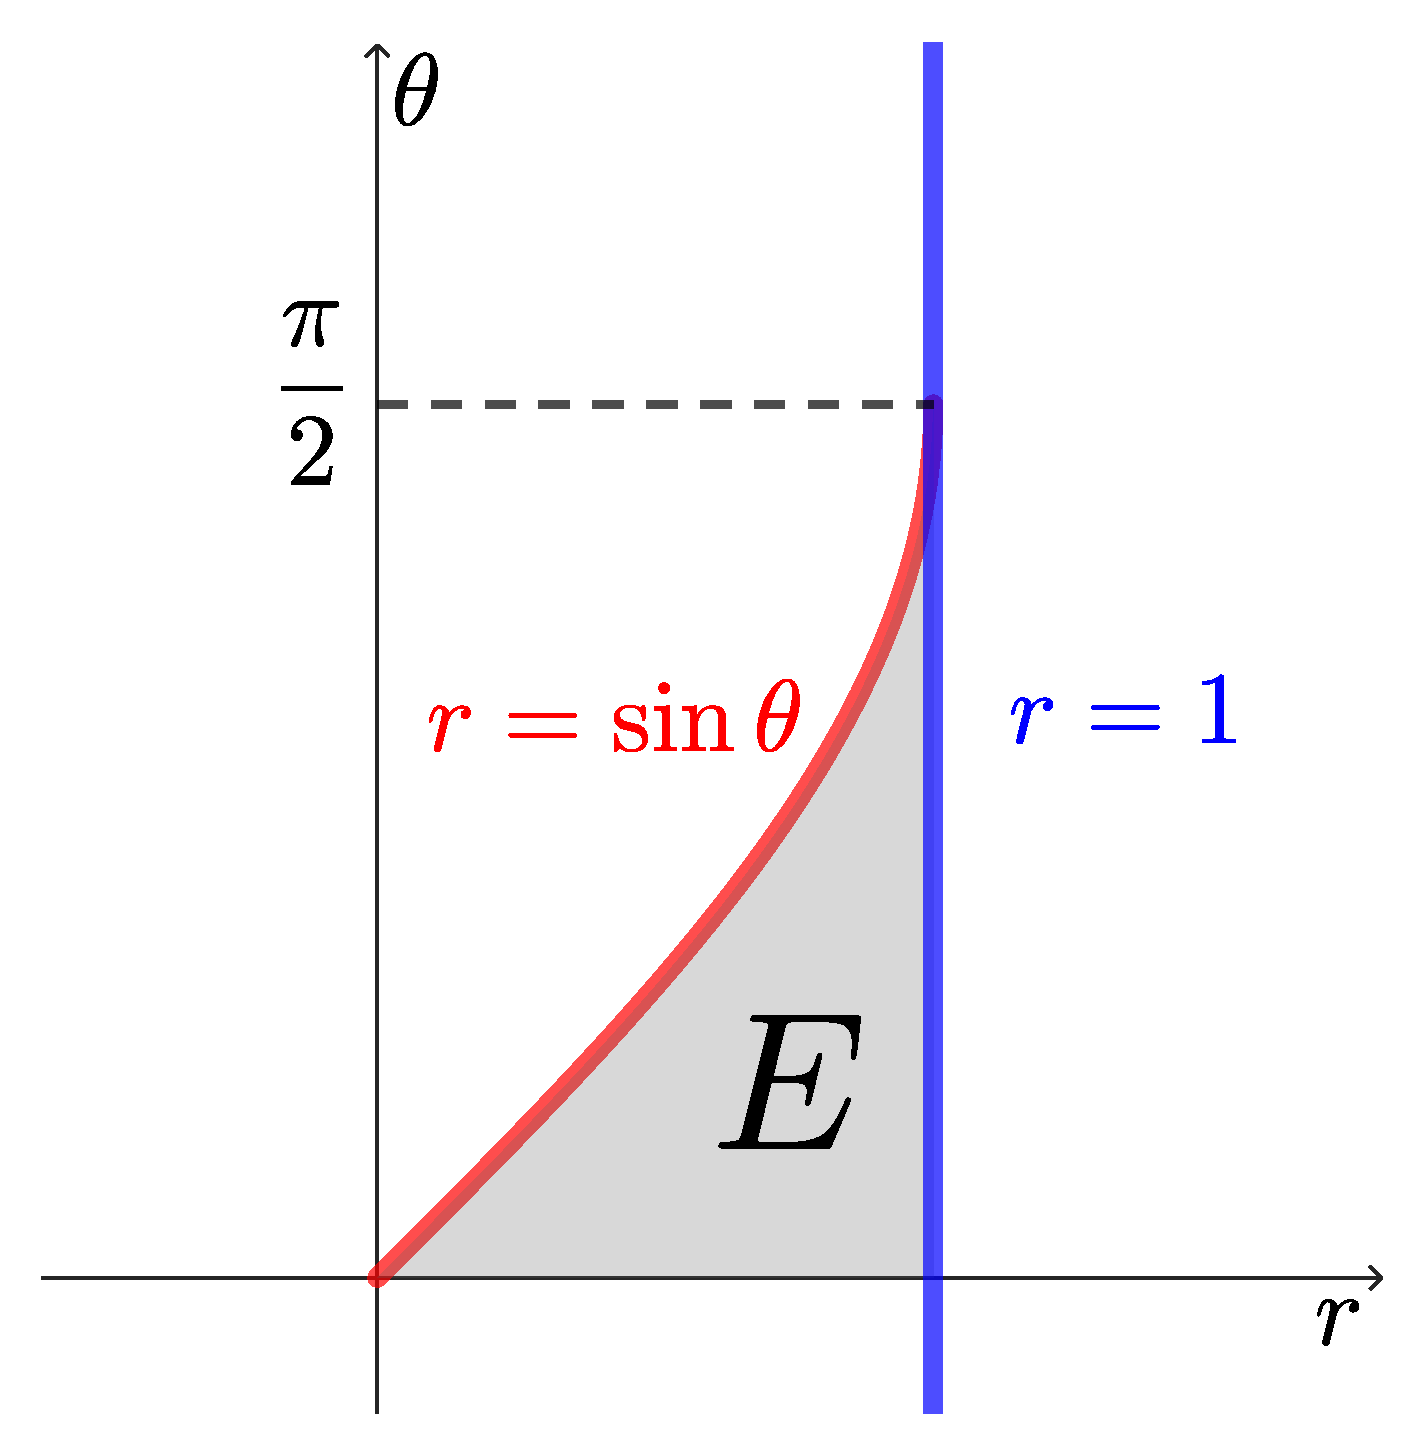
\includegraphics[height=6cm]{./pictures/fig3_rt.pdf} 
      &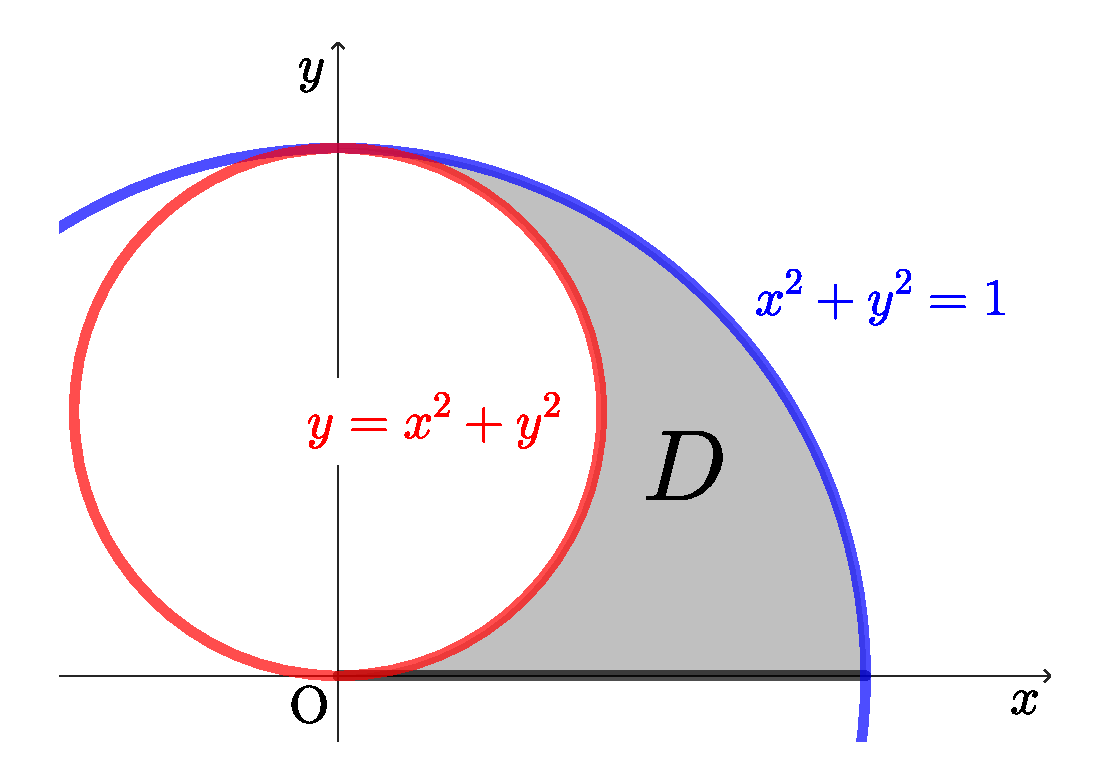
\includegraphics[height=6cm]{./pictures/fig3_xy.pdf}
    \end{tabular}
  \end{table}

  \newpage


\item $\ds \iint_{D}(x^2+y^2) \ dx dy, \quad D=\Set{(x,y) \ \mid \ \frac{x^2}{4} + \frac{y^2}{9} \leqq 1}$

  \vspace{1zh}

  変数変換 $
  \begin{cases}
    x = 2 r \cos \theta\\
    y = 3 r \sin \theta
  \end{cases}
  $ によって,$r\theta$ 平面の閉領域
  \[
    E= \Set{(r, \theta) \ \mid \ 0\leqq \theta \leqq 2\pi, \; 0 \leqq r \leqq 1}
  \]
  が $xy$ 平面の閉領域 $D$ に変換される.この変換の Jacobian は
  \[
    J(r, \theta) = \left|
      \begin{array}{rr}
        2 \cos \theta & -2r \sin \theta\\
        3 \sin \theta & 3r \cos \theta
      \end{array}
    \right| = 6r
  \]
  なので,2重積分は次のように計算できる.
  \[
    \begin{aligned}
      \iint_{D}\left( x^2+y^2\right) \ dx dy
      &= \iint_{E} r^2 \left| J(r, \theta)\right| \ dr d\theta
        = 6 \iint_{E} \left( 4\cos^2 \theta + 9 \sin^2 \theta\right) r^3 \ dr d\theta\\[1ex]
      & = 6 \left(\int_{0}^{2\pi} \left( 9 - 5\cos^2 \theta\right) \ d\theta\right)
        \left( \int_{0}^{1} r^3 \ dr\right) = \frac{39\pi}{2}
    \end{aligned}
  \]

  \begin{table}[h]
    \centering
    \begin{tabular}[h]{cc}
      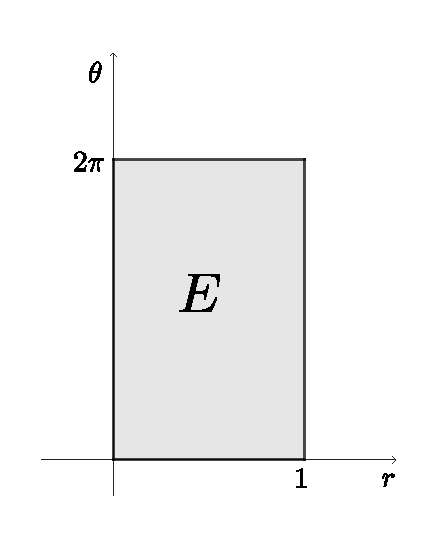
\includegraphics[height=8cm]{./pictures/fig4_rt.pdf} 
      &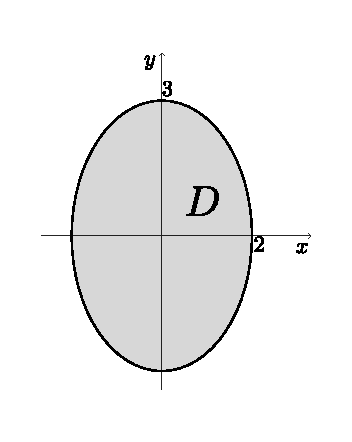
\includegraphics[height=8cm]{./pictures/fig4_xy.pdf}
    \end{tabular}
  \end{table}

  \newpage
  
\item $\ds \iint_{D} xy \ dx dy, \quad D=\Set{(x,y) \ \mid \ \sqrt{x}+\sqrt{y} \leqq 1}$
  
  \vspace{1zh}

  変数変換 $
  \begin{cases}
    x = u^2\\
    y = v^2
  \end{cases}
  $ によって,$uv$ 平面の閉領域
  \[
    E = \Set{(u,v) \ \mid \ u+v \leqq 1, \; 0 \leqq u \leqq 1, \; 0 \leqq v \leqq 1}
  \]
  が $xy$ 平面の閉領域 $D$ に変換される.この変換の Jacobian は
  \[
    J(u,v) = \left|
      \begin{array}{cc}
        2u & 0\\
        0 & 2v
      \end{array}
    \right| = 4uv
  \]
  なので,2重積分は
  \[
    \iint_{D} xy \ dx dy = \iint_{E} u^2 v^2 |J(u,v)| \ du dv = \iint_{E} 4 u^3 v^3 \ du dv
  \]
  と書き換えられる.ここで,$E$ は縦線集合として
  \[
    E = \Set{(u,v) \ \mid \ 0 \leqq u \leqq 1, \; 0 \leqq v \leqq 1-u}
  \]
  と書けるので,最終的に2重積分は次のように計算できる.
  \[
    \iint_{D} xy \ dx dy =  \int_{0}^{1} u^3 \left( \int_{0}^{1-u}4 v^3 \ dv \right) du
    =  \int_{0}^{1} u^3 \left( 1-u\right)^4 \ du = \frac{1}{280}
  \]

  \begin{table}[h]
    \centering
    \begin{tabular}[h]{cc}
      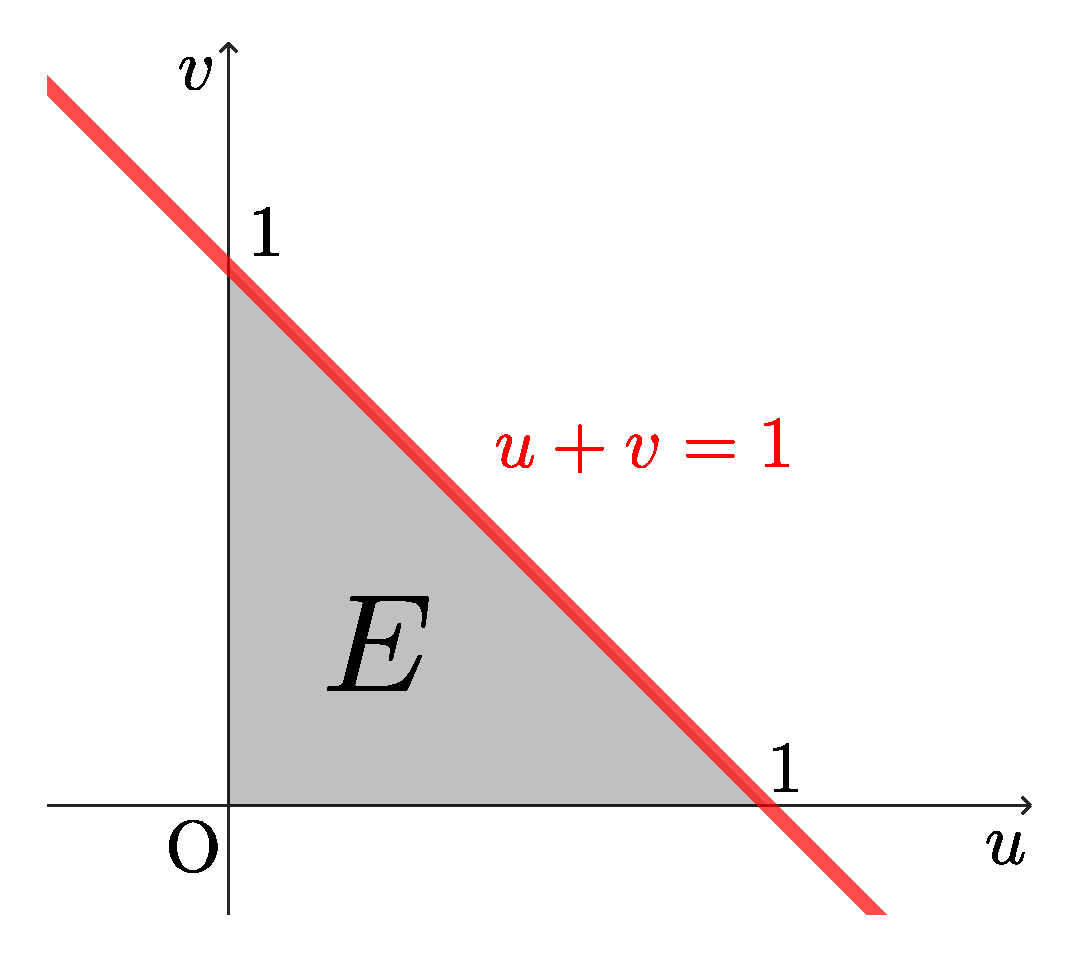
\includegraphics[height=6cm]{./pictures/fig5_uv.pdf} 
      &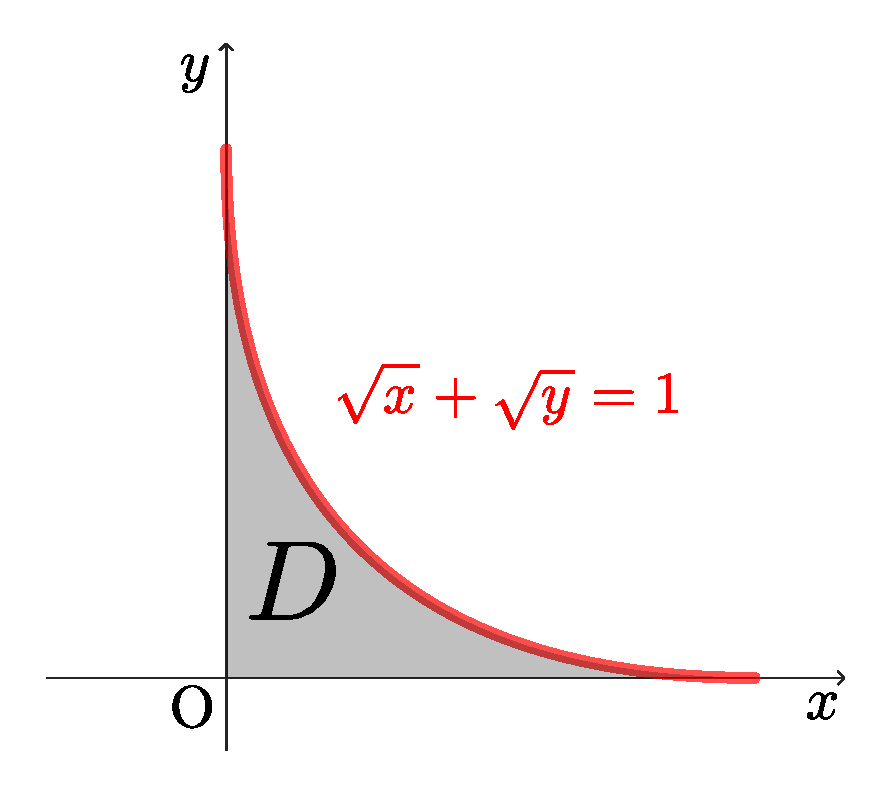
\includegraphics[height=6cm]{./pictures/fig5_xy.pdf}
    \end{tabular}
  \end{table}

\end{enumerate}



\end{document}

